\documentclass[]{article}
\usepackage{lmodern}
\usepackage{amssymb,amsmath}
\usepackage{ifxetex,ifluatex}
\usepackage{fixltx2e} % provides \textsubscript
\ifnum 0\ifxetex 1\fi\ifluatex 1\fi=0 % if pdftex
  \usepackage[T1]{fontenc}
  \usepackage[utf8]{inputenc}
\else % if luatex or xelatex
  \ifxetex
    \usepackage{mathspec}
  \else
    \usepackage{fontspec}
  \fi
  \defaultfontfeatures{Ligatures=TeX,Scale=MatchLowercase}
\fi
% use upquote if available, for straight quotes in verbatim environments
\IfFileExists{upquote.sty}{\usepackage{upquote}}{}
% use microtype if available
\IfFileExists{microtype.sty}{%
\usepackage{microtype}
\UseMicrotypeSet[protrusion]{basicmath} % disable protrusion for tt fonts
}{}
\usepackage[margin=1in]{geometry}
\usepackage{hyperref}
\hypersetup{unicode=true,
            pdftitle={Neuron Specificity},
            pdfauthor={Rasmus Munter},
            pdfborder={0 0 0},
            breaklinks=true}
\urlstyle{same}  % don't use monospace font for urls
\usepackage{graphicx,grffile}
\makeatletter
\def\maxwidth{\ifdim\Gin@nat@width>\linewidth\linewidth\else\Gin@nat@width\fi}
\def\maxheight{\ifdim\Gin@nat@height>\textheight\textheight\else\Gin@nat@height\fi}
\makeatother
% Scale images if necessary, so that they will not overflow the page
% margins by default, and it is still possible to overwrite the defaults
% using explicit options in \includegraphics[width, height, ...]{}
\setkeys{Gin}{width=\maxwidth,height=\maxheight,keepaspectratio}
\IfFileExists{parskip.sty}{%
\usepackage{parskip}
}{% else
\setlength{\parindent}{0pt}
\setlength{\parskip}{6pt plus 2pt minus 1pt}
}
\setlength{\emergencystretch}{3em}  % prevent overfull lines
\providecommand{\tightlist}{%
  \setlength{\itemsep}{0pt}\setlength{\parskip}{0pt}}
\setcounter{secnumdepth}{0}
% Redefines (sub)paragraphs to behave more like sections
\ifx\paragraph\undefined\else
\let\oldparagraph\paragraph
\renewcommand{\paragraph}[1]{\oldparagraph{#1}\mbox{}}
\fi
\ifx\subparagraph\undefined\else
\let\oldsubparagraph\subparagraph
\renewcommand{\subparagraph}[1]{\oldsubparagraph{#1}\mbox{}}
\fi

%%% Use protect on footnotes to avoid problems with footnotes in titles
\let\rmarkdownfootnote\footnote%
\def\footnote{\protect\rmarkdownfootnote}

%%% Change title format to be more compact
\usepackage{titling}

% Create subtitle command for use in maketitle
\newcommand{\subtitle}[1]{
  \posttitle{
    \begin{center}\large#1\end{center}
    }
}

\setlength{\droptitle}{-2em}
  \title{Neuron Specificity}
  \pretitle{\vspace{\droptitle}\centering\huge}
  \posttitle{\par}
  \author{Rasmus Munter}
  \preauthor{\centering\large\emph}
  \postauthor{\par}
  \predate{\centering\large\emph}
  \postdate{\par}
  \date{May 11, 2018}

\usepackage{float}

\begin{document}
\maketitle

\section{Project 1}\label{project-1}

The goal of this project was to look for a relation between neuron
firing and the head angle of a mouse. The dataset consists of finished
data from tetrodes in a mouse brain and has been preprocessed to extract
the activations of individual neurons. To constrain the data amount the
following subset of data was used:

\begin{itemize}
\tightlist
\item
  Session 131213 on mouse 24
\item
  Session 140124 on mouse 25
\item
  Session 140318 on mouse 28
\end{itemize}

The mouse head angle was binned into 40 bins giving bins of length 9. To
find neurons with a relation the binned angle was plotted against the
corresponding average firing rate. Then, manually, any neurons that
seemed to have a bump in activity that clearly stood out among the
firing activity noise was noted. An example of the plots used to find
these follows.

\subsection{Visualising cells}\label{visualising-cells}

\begin{center}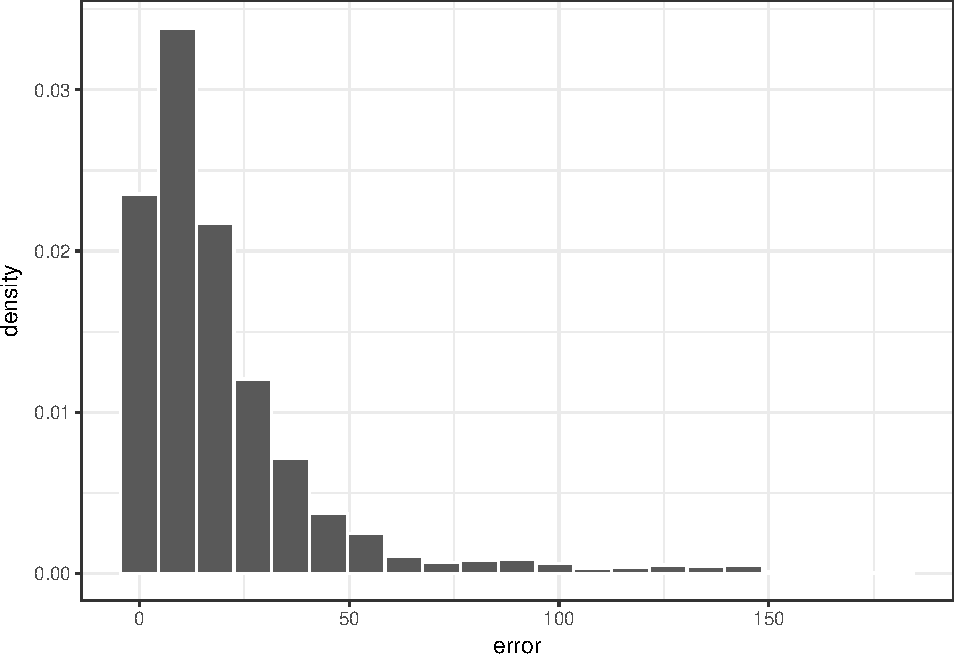
\includegraphics{project1_files/figure-latex/unnamed-chunk-5-1} \end{center}

The following cells were found to have distinct peaks.

\begin{center}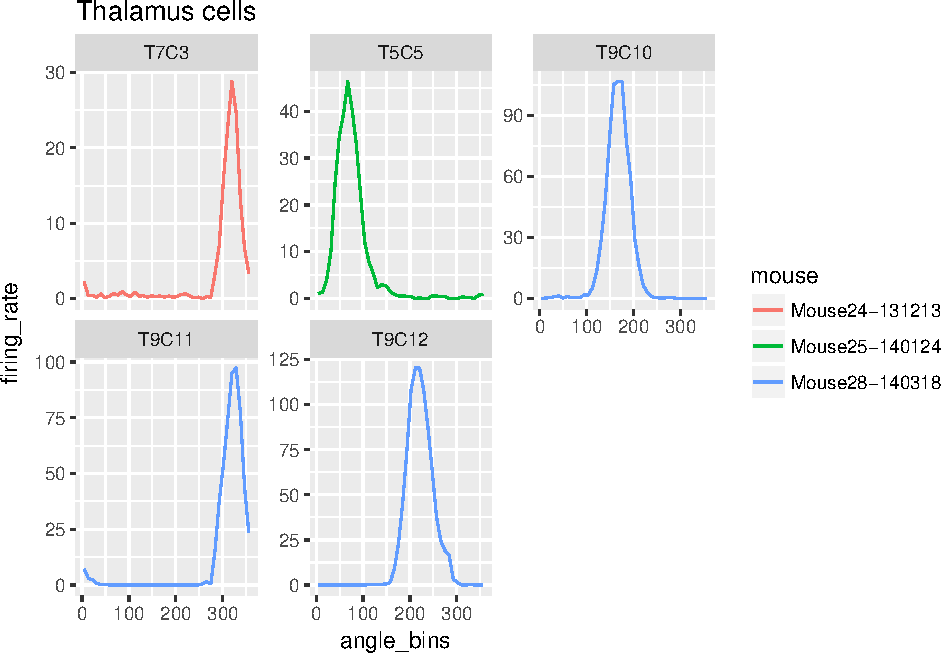
\includegraphics{project1_files/figure-latex/unnamed-chunk-13-1} \end{center}

\begin{center}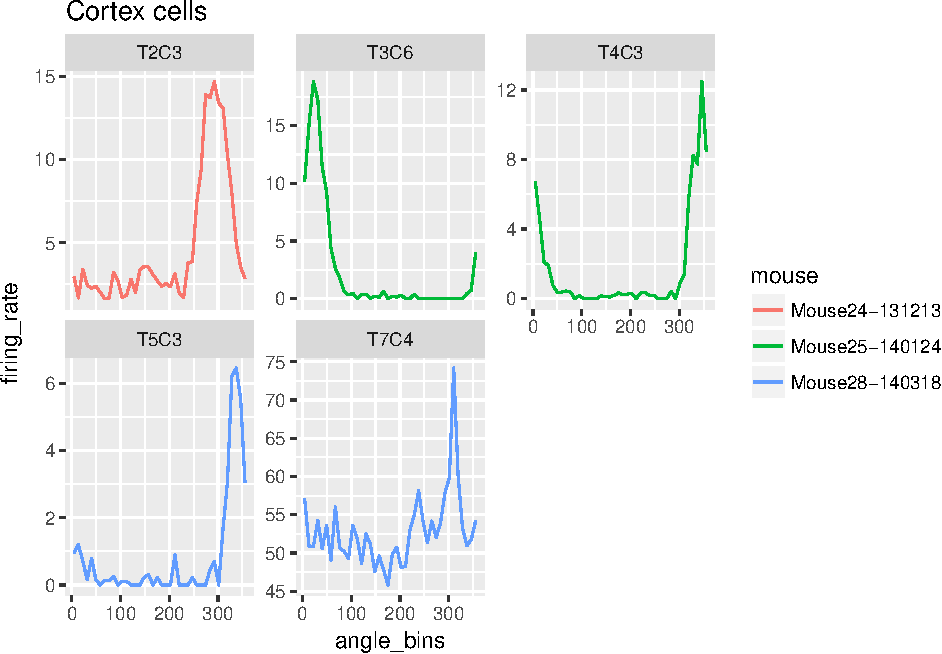
\includegraphics{project1_files/figure-latex/unnamed-chunk-13-2} \end{center}

In the thalamus there were relatively many neurons with distinct peaks.
This is to be expected as the thalamus is an area known to have head
direction cells and head direction cells are known to have distinct
peaks. The subiculum is also supposed to have head direction cells but
in general these had more background noise and sharper peaks.

\%\% Page 290 in the book

For use in further projects the total number of neurons had to be
restricted to 10 neurons. The following neurons were chosen from the
thalamus and cortex respectively.

\begin{center}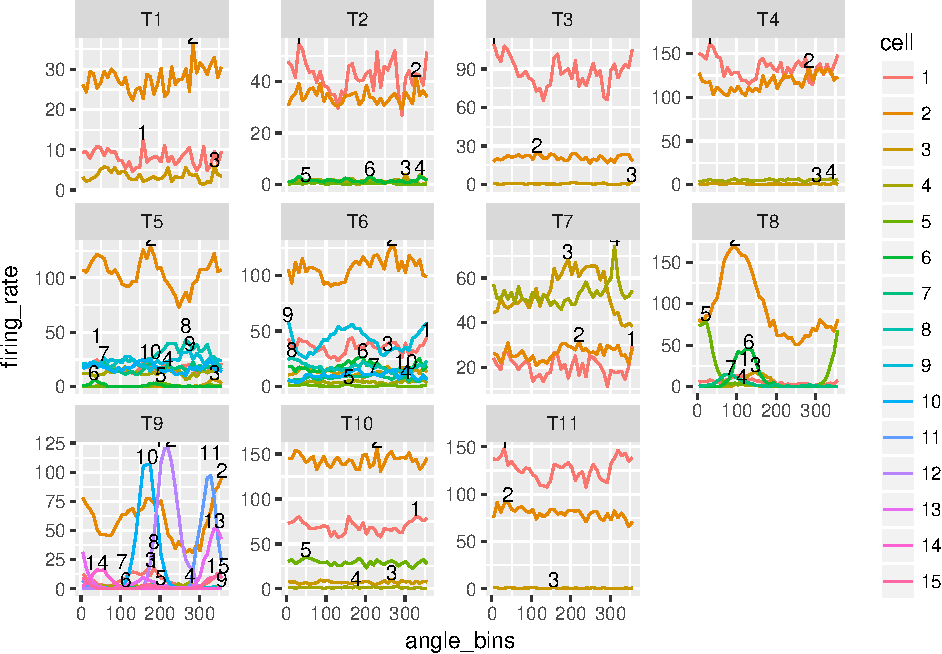
\includegraphics{project1_files/figure-latex/unnamed-chunk-14-1} \end{center}

\begin{center}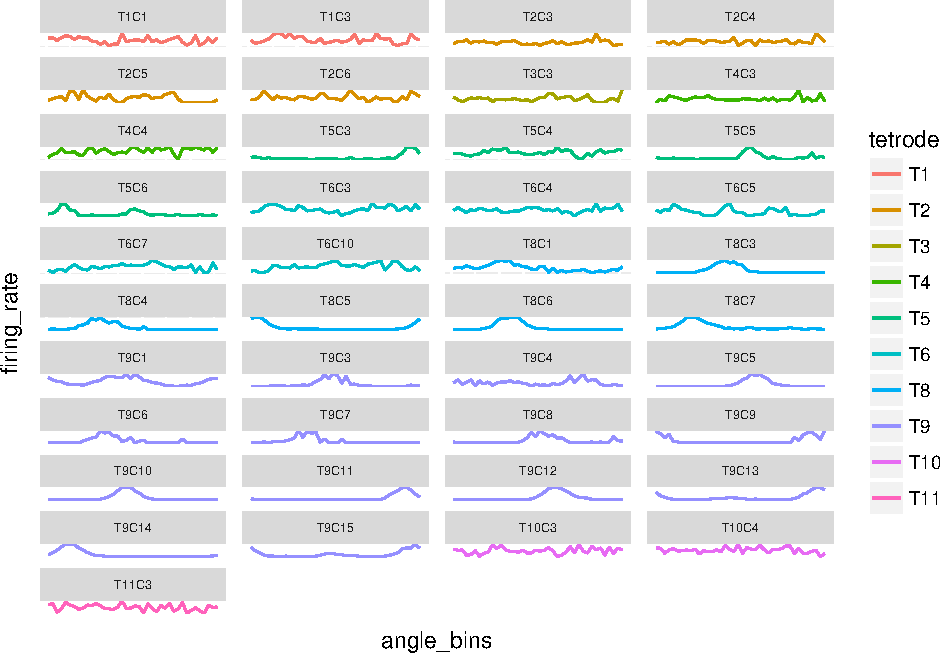
\includegraphics{project1_files/figure-latex/unnamed-chunk-14-2} \end{center}


\end{document}
